\section{BACKGROUND}

\subsection{ACH (Shared Memory)}

POSIX IPC offers three types of messages: streams, datagrams and shared memory. For the real time robotics application, it is important to ensure that the IPC system is non head of line blocking as the most recent sensor data will take priority over previously acquired data. Streams suffers from head of line blocking and is thus not a desirable method for robotics. Datagrams utilize a data buffer that when full, loses any new data. This is particularly problematic as the robot would routinely lose important data. Shared memory is the fastest method of the POSIX suite and will provide the most current data by overwriting any old information stored. Unfortunately this method is susceptible to synchronization issues and further considerations must be taken in code which would reduce its reusability and complexity. Furthermore, for a realtime system, none of the POSIX IPC methods allow any methods of priority inheritance which is critical to allow high priority systems to access data first.

%\begin{figure}
%	\caption{HUBO ACH Flow Chart}
%	\centering
%		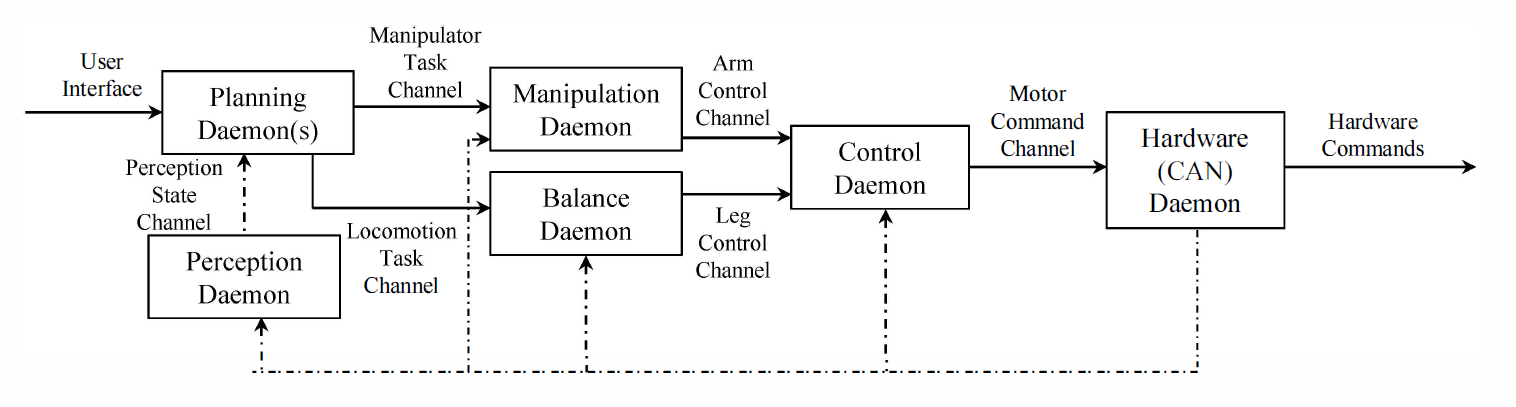
\includegraphics[width=0.5\textwidth]{./images/achflow.png}
%\end{figure}

\begin{figure}[thpb]
 \centering
 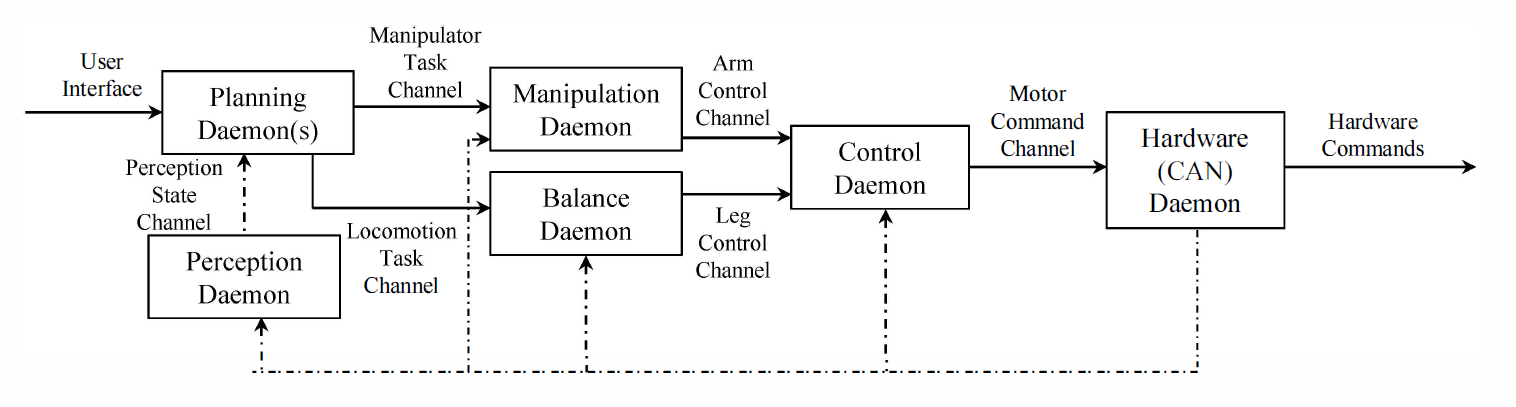
\includegraphics[width=1.0\columnwidth]{./images/achflow.png}
  \caption{HUBO ACH Flow Chart}
  \label{fig:archr-sys-diagram}
\end{figure}

The ACH system allows the system to create multiple data channels to send data between processes. Each channel consists of two circular buffers: a data buffer and an index buffer. The two buffers are written in a channel specific POSIX shared memory file. By storing the data buffers in shared memory, the synchronization issue can be solved once for the entire channel via a mutex, allowing each reader process to poll the channel or wait for new data to be posted. This also prevents starvation and allows for priority inheritance between the real time processes.

A case study is presented \cite{REALTIMEACH} in which a balancing bipedal robot was developed with many different processes and ACH channels. The study details how the multiprocess approach allows for high priority processes (like balancing in this case) to stay alive in the event that other processes fail (ie computer vision). This approach also allowed processes to be distributed between smaller microcontrollers to drive servomotors to higher powered computers to process computer vision. For the 

SPIN simulations were run to benchmark the ACH system and it was shown that performance is identical to POSIX for single readers and receivers and the majority of the latency is a product of context switches. 

Due to ACH relying on shared memory, it is not a system that can be used on its own if the system requires networked communications. This can be resolved by using a sockets (TCP/UDP) communication method to send data across the network to an ACH channel\cite{ACHHUBO}. This method allows for CPU intensive processes to be offloaded from the robot to a local high performance computer, maintains the non head of line blocking nature of the ACH channel, and all other processes running on the robot now have access to the most recent data sent without processing any messages sent before it.

\subsection{Sockets: TCP and UDP}

Sockets provides interprocess communication over a network via the TCP (Transmission Control Protocol) and UDP (User Datagram Protocol). The implementations evaluated for this paper are the client/server  architecture, which provides one to one communication between processes. Both TCP and UDP operate over a network interface and are bound to a specific port number and IP address. Wireless networks and wireless connected devices have become ubiquitous in modern society. With the growing number of single board computers with full ethernet/wireless network interfaces, it is possible to quickly and cheaply set up a robotic system that can interact with sensors, high power computers, and external controllers. Sockets is a well seasoned IPC and can be found as part of the POSIX library, allowing for many different operating systems and programming languages to communicate with no extra software and little programming effort. With modern newtork routers offering gigabit connections, sockets can provide a method of fast communication between processes distrubted across a network. 

\subsubsection{TCP}

TCP offers a faily robust communication link between a single client and a single server process. When created, the two processes will perform some handshaking to complete the connection. During each transmission from a client, there is a response from the server indicating if the message was received. This allows the system to identify if a message was not sent. For many applications this would be an advantage, but in robotics data can be streaming in from sensors at a high rate and the missed message would be obsolete by the time the system realizes the missed transmission\cite{UDPTCP}. Any retransmission would add additional delay on top of the delay incured by waiting for a response from the server.

A TCP server receives messages as they arrive in the buffer and must process each message in the order it is sent. This first in first out system (FIFO) allows for all messages to be saved, but again suffers from the disadvantage of older messages beingn prioritized over new. If message are being received at a higher frequency than a process is running, the process must consume all old data received while alseep before accessing the data that is in real time.

\subsubsection{UDP}

UDP offers one quick directional communication from a client process to a server process. Each process is bound to a target IP address and port number. There is no handshaking or direct link between the processes. This allows mutltiple clients to send data to a single server. As there is no response indicating a successful transmission of a message, UDP inherently has less latency than TCP. The disadvantage to this method is that if all data is of critical importance, message can be missed and the system has no way of identifying that data was lost. Depending on the application, the requirement of high speed data transmission can overcome the tradeoff for message transmission assurance.

\subsection{ZeroMQ}

ZeroMQ (ØMQ) is a messaging system that extends on the foundations of sockets. It provides an additional abstraction layer over TCP by sending messages to a system topology instead of specific IP addresses. ØMQ prevents sending to specific IP addresses by design. The available messaging patterns is open ended, popular systems include publish/subscribe and request/reply. Only one messaging pattern is allowed for a topology and they cannot be interconnected. This is essential to providing guarantees that data will arrive at its intended location. ØMQ separates its stack into end to end and hop by hop layers. Unlike TCP/IP, each ØMQ end to end protocol has its own hop by hop protocol\cite{ZMQTHEORY}. This allows each specific messaging pattern to have their own routing functionality. This allows bidirectional messages to be sent to specific nodes in the topology. Each intermediary node can determine if downstream sections of the network are unreachable and can signal the original client to resend now or wait until connectivity has been reestablished. 

With multicore processors being commonplace in today’s market and the growing availability of multicore processors in commercially available embedded systems there is a need for efficiently written multithreaded code. Current methods of dealing with the issues that arise from multithreading (synchronization, starvation, priority inversion) are difficult to learn and do not scale well as the number of available cores increases. By creating code with too many locks, threads can block one another and the system can perform inconsistently depending on what system the program is running on. Writing lock free code can become susceptible to processors reordering instructions and the code again performing inconsistently. These multithreading approaches are API based and incorrect usage can often result in multiple threads blocking each other and the program essentially running as a single threaded process. 
ZeroMQ provides a solution to these issues by abstracting the more difficult lock free multithreading code behind its native message passing techniques and achieves simple multithreading by sending messages between threads. Being based on BSD Sockets, the code implementation is simple and intuitive for existing programmers, as well as being available for a multitude of programming languages. ZeroMQ is infinitely scalable as the number of available cores increases without any rewriting of existing code.


\subsection{ROS}

ROS (Robot Operating System) is a flexible framwork for developing robotic systems. Despite its namesake ROS is not an operating system, and it offers more features than just an IPC. ROS utilizes TCP as its core transport mechanism for communication between its processes, but the architiecture differs than the TCP presented earlier as part of sockets. In addition to the IPC, ROS offers a wide library of prebuilt tools and a vast user base from which to draw on modular solutions that can plug into any ROS system. This reduces the development time and amount of low level code that needs too be written for each piece of hardware.

insert image here

With the growing availability of cheap ARM processor systems, versions of ROS are being developed to provide a lower cost design than the traditional full-fledged Linux pc. ROS subsystems can be distributed over multiple ARM systems, allowing for more design flexibility, lower power consumption, and improved scalability. ROS allows for higher level systems to be separated from real time subsystems and other system critical functions. This allows for high priority systems to be simplified to reduce risk of failure. ROS was designed to support higher level robot functions instead of the control of individual motors/sensors/etc. Much of the integration of subsystems is left to the design as ROS does not support fieldbuses. 
b
Three architecture styles exist for the designing to embed the ROS system: Embedded PC, Proprietary system with interface, or use of ROS messaging and APIs. The embedded PC would require all control hardware of subsystems to be fitted to the PC itself. This provides smooth integration with ROS, but fails to offer real hard time support. Entire existing robots can be managed from ROS by configuring a translation function between the proprietary system and the embedded system. This abstracts the lower level programming and allows for the existing systems to operate in real time. The third architecture is focused on the IPC system for ROS, which operates on remote procedure calls and publish/subscribe support. 

The ROS IPC system allows for custom messages to be used and provides flexibility in configuring the embedded systems. Rosserial, rosc, and Rosbridge are common methods of passing these messages. Rosserial provides a proxy over a C++ client that can be ported easily to any system that supports the language, not required an OS. Rosserial provides a ROS-like API to publish, subscribe, offer and consume RPC services. Potential issues arise with the proxy becoming a bottleneck. Rosc allows for direct connection to the Ethernet and handles native ROS connections and messages. However, for embedded systems, the TCP/IP overhead may prove too overwhelming for low powered systems. Rosbridge provides dynamic socket and websocket access to the full capabilities of ROS

The emphasis of robotics research has shifted from larger platforms to smaller low cost platforms. This paper evaluates two Arduino based robotic systems: TraxBot and StingBot for use in an educational  environment. Arduino provides a simple programming interfaces, highly available expansion/interfaces boards, and large online resources for sample code. ROS provides libraries and tools to be used across wide variety of hardware, allow for greater code reuse across different projects. ROS goals are to provide hardware abstraction, low level device control, easy implementation of common functionality, and message passing between processes. There are many commercially available robotic platforms (Roomba, lego mindstorms, etc) that can be cheaply obtained and have ROS drivers publically available. Existing commercial platforms offer little hardware expandability, but the growing Arduino community would solve this issue. 
The normal rossearial interface used for Arduino projects has high overhead and result in an excessive workload for the processor evaluated (Atmel 328P). For this Arduino system, the SRAM limitations provided a maximum of only 15 standard ROS topics to be used in parallel and the message buffer was limited to 70 standard messages. To circumvent this problem, the researchers developed a custom ROS driver that utilizes serial communications where ROS messages sent from the arduino are represented by character arrays. Translation can take place on the more powerful PC running the ROS core. There is a separate ROS node running to interface with the custom serial packet developed. By using this node/driver combination to integrate any Arduino platform, the benefits of existing Arduino hardware can be easily implemented in any existing ROS system. Regardless if the project is small or spans multiple teams in multiple locations. 





